\chapter{Machine Learning Basics}
Bayesian neural networks are a specific kind of neural network which is a type of machine learning algorithms. So in order to understand Bayesian neural networks one must first know the basic principles of machine learning. This chapter provides a brief introduction to the fundamental theory of machine learning, that is used throughout the rest of this dissertation. \\
\\
Machine learning is the study of computer algorithms that learn by analyzing data. Most machine learning algorithms can be divided into the two categories of supervised learning and unsupervised learning. We describe the informal distinction between these and the most common tasks used for supervised learning. As neural networks are considered supervised learning the following sections focuses only on theory for supervised learning algorithms.\\
\\
We proceed to describe the challenge of finding patterns and generalizing these to new data while describing the various machine learning components such as capacity, loss functions and regularization. Most machine learning algorithms are based on the idea of minimizing the loss function using an optimization algorithm. One of the most common optimization algorithms used in the context of machine learning is called stochastic gradient descent, which we cover in section \ref{sec:sgd}. We will later use the theory of stochastic gradient descent in combination with backpropagation in section \ref{sec:backprop} for describing learning in neural networks.\\
\\
As machine learning is a form of applied statistics that focuses on computer algorithms to make statistical estimates we present the two central approaches to statistics: frequentist estimators and Bayesian inference, with emphasis on the latter as this is the approach used in Bayesian neural networks.

\section{Supervised learning}
Machine learning algorithms are typically categorized by being either supervised or unsupervised. Supervised learning use labelled examples as targets to create prediction rules (also called hypothesis) for learning the label of new examples. Unsupervised learns useful properties of the structure of the data without being provided target labels to predict. However as mentioned by \cite{Goodfellow-et-al-2016} the distinction is not formally defined since there is no objective way to determine whether a value is a feature or a target label.\\
\\
One example of a learning algorithm that is typically viewed as supervised is classic linear regression that uses examples $x$ and their labels $y$ to create a linear function to determine $y$-values of new examples $x$. An example of a learning algorithm one typically views as unsupervised is $k$-means clustering, that divides a training set into $k$ clusters based on the distance of the examples. \\
\\
As Bayesian Neural Networks uses target labels to predict labels of new examples it is considered a supervised learning algorithm. Therefore the following chapter will only cover the machine learning basics of supervised algorithms. \\
\\
Typical tasks of supervised machine learning algorithms are:
\begin{itemize}
    \item Classification when the output space $\YY$ are labels. This is called binary classification when we work with 2 labels. In this case the algorithm must learn to separate examples of these 2 labels. Binary labels (be it male or female, yes or no etc.) are typically translated to a numerical representation by taking $\YY = \{ \pm 1 \}$ or $\YY = \{0,1 \}$. When working with more than 2 but a finite amount of labels we call the task multiclass classification. Depending of the setting and amount of labels it can be preferable to use regression instead of multiclass classification.
    \item Regression when the output space $\YY = \mathbb{R}$. For example predicting someones weights could be modeled as a regression problem.
    \item Structured prediction when the output is not merely a number or a label, but a structured object. An example of this is machine translation where the input is a sentence in one language and the output a sentence in another language. 
\end{itemize}


\section{Loss Functions} \label{sec:loss_func}
In order to evaluate the performance of a supervised machine learning algorithm we use a quantitative measure called a loss function. The loss function is an encoding, of how much the algorithm should care about making certain kinds of mistakes, and it is based on this measure that the algorithm selects a hypothesis $h$ from a set of possible hypothesis $\mathbb{H}$ called the hypothesis space. A hypothesis (also called prediction rule) can be understood as a recipe, that the algorithm develops to perform it's task. An example would be the weights $\boldsymbol{w}$ for performing the linear regression $\hat{y}^{(i)} = \boldsymbol{w}^\top \boldsymbol{x}^{(i)}$. Another example would be a specific range of values for a specific set of features for classification, like a set of RGB color-values to classify if an input-image is depicting an apple or a pear. We treat the hypothesis as a function $h\lr{\boldsymbol{x}^{(i)}}$ taking $\boldsymbol{x}^{(i)}$ as input and predicting $\hat{y}^{(i)}$. We define the loss function $\ell \lr{h \lr{\boldsymbol{x}^{(i)}}, y^{(i)}}$ as being the loss of predicting $h \lr{\boldsymbol{x}^{(i)}}$ when the target label is $y^{(i)}$.\\ 
\\
We want the algorithm to return the "best" hypothesis $h^*$, which in this context should be interpreted as the hypothesis that gives the least amount of expected loss on new samples $\lr{\mathbf{x}^{(i)}_{\text{new}}, \text{y}^{(i)}_{\text{new}}}$
\begin{equation*}
    L(h) \equiv \E \lrs{\ell \lr{h \lr{\mathbf{x}_{\text{new}}^{(i)}}, \text{y}_{\text{new}}^{(i)}}}
\end{equation*}
where the expectation is taken with respect to the data distribution $p_{\text{data}}$. If such a value is satisfyingly low, it means that $h^*$ is a useful tool for performing its task on new data. We write this formally as
\begin{equation*}
   h^* = \argmin_{h \in \mathbb{H}} L(h)
\end{equation*}
\\
A typical loss function used for binary classification is the zero-one loss 
$$ \ell\left(h\lr{\boldsymbol{x}^{(i)}}, y^{(i)}\right)=\1\left(h\lr{\boldsymbol{x}^{(i)}} \neq y^{(i)} \right)=\left\{\begin{array}{ll}
0, & \text { if } h\lr{\boldsymbol{x}^{(i)}}=y^{(i)} \\
1, & \text { otherwise }
\end{array}\right. $$
giving $0$ loss for when the predicted label $h\lr{\boldsymbol{x}^{(i)}}$ is equal to the true label $y^{(i)}$ and $1$ otherwise. This loss function trains the algorithm to generate hypothesis, that makes the least number of mistakes. \\
\\
Common loss functions in regression are squared loss (also called L2 loss)
\begin{equation} \label{eq:mse}
    \ell\left(h\lr{\boldsymbol{x}^{(i)}}, y^{(i)} \right) = \lr{ h\lr{\boldsymbol{x}^{(i)}} - y^{(i)} }^2
\end{equation}
or absolute loss (also called L1 loss)
$$ \ell\left(h\lr{\boldsymbol{x}^{(i)}}, y^{(i)}\right) = \lra{h\lr{\boldsymbol{x}^{(i)}} - y^{(i)}}$$
These functions trains the algorithm to create hypothesis that minimizes the differences from the target labels. \\
\\
A loss function used in a Bayesian setting is the Kullback-Leibler (KL) divergence
\begin{equation}\label{eq: KL}
    D_{\mathrm{KL}}(P \| Q)=\mathbb{E}_{\mathrm{x} \sim P}[\ln P(x)-\ln Q(x)]
\end{equation}
This function measures how different two distributions $P(x)$ and $Q(x)$ are over the same random variable $x$. The KL divergence has the useful properties of being non-negative and equal to $0$ if and only if $P$ and $Q$ are the same distribution for discrete variables and equal to $0$ almost everywhere for continuous variables. \cite{Goodfellow-et-al-2016} shows how the KL divergence is not symmetric $D_{\text{KL}}(P \| Q) \neq D_{\text{KL}}(Q \| P)$ meaning that there are important consequences to the choice of using $D_{\text{KL}}(P \| Q)$ or $D_{\text{KL}}(Q \| P)$. \textcolor{red}{Revisit.}
\\
\\
These are some of the convenient general choices, and there are many more. But such general loss functions is not necessarily the right choice for a particular application. For example if a firm knows the exact monetary loss of packing a wrong item as a result of a misclassification happening in a robotic packaging system. Then it might be beneficial to use a table (perhaps formally written as a sum of indicatorfunctions) of the costs of packaging each of their items as a loss function instead of using the general ones found in the literature.
\textcolor{red}{ADD A PART ABOUT CROSS-ENTROPY HERE}.
\section{Training \& Validating} \label{sec:train_val}
The central challenge in machine learning is making sure the algorithm creates hypothesis that perform well on new data that was not used in selecting the hypothesis. As mentioned in section \ref{sec:loss_func} this is done by minimizing $L(h)$, but as we don't know $p_\text{data}$ (if we did we wouldn't need the algorithm) we can't evaluate $L(h)$. We must instead approximate $L(h)$ by it's empirical estimate 
\begin{equation*}
    \hat{L}(h,S)= \frac{1}{N} \sum_{i=1}^N \ell \lr{h\lr{\boldsymbol{x}^{(i)}}, y^{(i)}}
\end{equation*}
with $\lr{ h\lr{\mathbf{x}^{(i)}}, \text{y}^{(i)}} \in S$ for $i = 1, \dots N$.\\
\\
However when we select a hypothesis $\hat{h}^*_S$ in $\mathbb{H}$ based on empirical loss $\hat{L} \lr{h, S}$ then the loss of this hypothesis $\hat{h}^*_S$ becomes a biased estimate of $L(\hat{h}^*_S)$. This is because $\hat{h}^*_S$ is selected based on the minimum empirical error on $S$, so from the perspective of $\hat{h}^*_S$ new samples might not be interchangeable with samples in $S$, since including these new samples could result in a different hypothesis that minimizes the loss on $S$. \\
\\
To get an unbiased estimate of $L(\hat{h}^*_S)$ for evaluating a model it is common practice to split the sample set $S$ into a training set $S_\text{train}$ and a validation $S_\text{val}$. One can then find the best hypothesis for the training set $h^*_\text{train}$ and use the validation set for computation of $\hat{L}\lr{h^*_\text{train}, S_\text{val}}$ which he can then used to evaluate the performance. Based on the assumption that new samples $\lr{\mathbf{x}^{(i)}_{\text{new}}, \text{y}^{(i)}_{\text{new}}}$ are distributed identically with the samples in $S_\text{val}$ then these new samples are exchangeable with the ones in $S_\text{val}$ from the perspective of $h^*_\text{train}$. This means that $\E \lrs{\ell \lr{h^*_\text{train} \lr{\boldsymbol{x}^{(i)}}, \boldsymbol{y}^{(i)}}} = \E \lrs{\ell \lr{h^*_\text{train} \lr{\mathbf{x}^{(i)}_{\text{new}}}, \text{y}_{\text{new}}^{(i)}}}$ and therefore $\hat{L}\lr{h^*_\text{train}, S_\text{val}}$ is an unbiased estimate of $L(h^*_\text{train})$.

\subsection{Cross-Validation} \label{sec:cv}
Splitting a dataset into a training set and a validation set can be problematic if the resulting validation set is too small. Such a small validation set will give rise to statistical uncertainties around the estimated average loss and will make it problematic to evaluate the model. When we have large dataset this is not a problem, but when we work with small datasets it can become a serious issue. \\
\\
A workaround for this issue is to use cross-validation. Cross-validation repeats the training and testing procedure on different randomly chosen splits of the original dataset. This enables us to use more examples for estimating the average test loss for the cost of computational power. This approach is also useful for choosing hyperparameters like regularization constants $\alpha$ covered in section \ref{sec:regularization}.\\
\\
A common method for cross-validation is the $K$-fold cross-validation that splits the dataset into $K$ non-overlapping and roughly equally sized subsets. On trial $i$ the $i$th subset is used as the validation set while the rest $K - 1$ subsets is used as the training set. The validation loss is then estimated by the cross-validation loss computed as the average validation loss across the $K$ trials.\\
\\
One problem with this approach is however measuring the uncertainty since there is no unbiased estimators of the variance of the average error estimators as mentioned by \cite{Bengio04}, so one must instead use approximations. Another discussed issue is how the choose the value for $K$. This problem does not have a clear answer but 5- or 10-fold cross-validation are generally recommended as a good compromise, see \cite{brieman_spector_1992} and \cite{kohavi_1992}.

\section{Overfitting \& Underfitting}
The average loss attained on the training set when selecting the best hypothesis $\hat{L}\lr{h^*_\text{train}, S_\text{train}}$ is what we will call the training error. The average loss attained from the validation set $\hat{L}\lr{h^*_\text{train}, S_\text{val}}$, used for validating the model, is what we will call validation error.\\
\\
Having a low training error means that we have made a prediction rule that fit our training set well. Having a small gap between training and validation error means that the prediction rule generalizes well on new data, which is why the validation error is also sometimes called generalization error. These factors are what corresponds to underfitting and overfitting, which is used to measure performance of the model.\\
\\
Underfitting occurs when the model is not able to obtain a sufficiently low training error. This is seen in figure \ref{fig:regr_example} in the case of linear regression of degree 1, where the model fitted on the training data lies far from the training samples, meaning it must have a large mean square training error. Overfitting occurs when the gap between the training error and validation error is too large. This large gap indicates that the model faithfully reflects idiosyncrasies of the training data rather than the true underlying process generating the data. This can be seen in figure \ref{fig:regr_example} in the case of linear regression of degree 15, where the model lies very close to all of the training samples meaning it must have a very small mean square training error. But if we sample points from the true function we see that many of these very likely will lie far from the model, thus resulting in a large test error relative to the training error. Overfitting and underfitting are both something we want to avoid. \\
\\
We can control whether a model under- or overfits by changing it's capacity. Capacity is a model's ability to learn a larger variety of hypothesis. A model with a low capacity might underfit the training set if it can't capture the structure of the data. A model with high capacity might overfit if it learns properties of the training set that isn't representative of the validation set. As an example we can increase the capacity of linear regression by allowing it to fit higher order polynomials, thus increasing the hypothesis space from which we draw prediction rules. This example is seen in figure \ref{fig:regr_example}, where we see that a low capacity causes underfitting while a very large capacity causes the model to overfit.

\begin{figure}[h!]
    \centering
    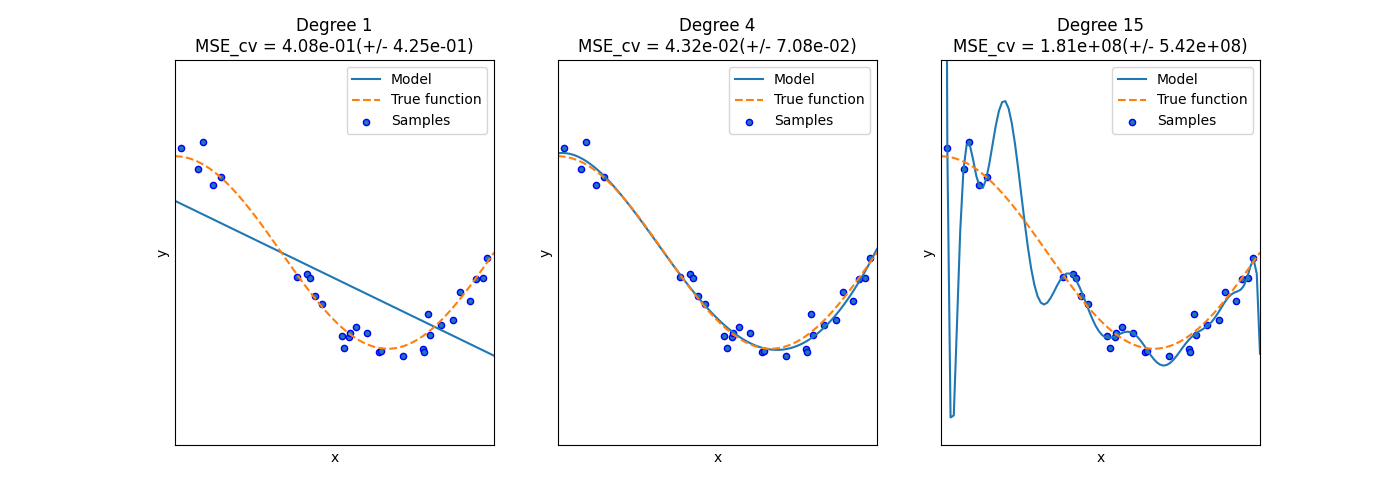
\includegraphics[width=\textwidth,height=\textheight,keepaspectratio]{reg_example.png}
    \caption{Regression of different degree polynomials on a $\cos$ curve. We see that a linear regression of degree 1 is insufficient to fit the training set and is underfitting. A polynomial of degree 4 fits the curve almost perfectly while a polynomial of degree 15 learns the noise of the data and overfits. How well the different regressors generalize to a validation set is evaluated quantitatively by calculating the mean square error using the loss function in equation \ref{eq:mse} using 10-fold cross-validation. We see that this error is lowest when using 4-degree polynomial regression. Cross-validation is covered in section \ref{sec:cv}. The standard error of these losses are shown in the parenthesis.}
    \label{fig:regr_example}
\end{figure}
\noindent
\textcolor{red}{Perhaps add some text on Bias \& Variance and how these are somewhat correlated to over-underfitting.}

\section{Regularization}\label{sec:regularization}
So far we have covered how to control over- and underfitting by changing a model's capacity. Another method is regularization which encodes the objective function with preferences for certain functions instead of excluding functions from the hypothesis space. The objective function is what we ask a machine learning algorithm to minimize, and has in the previous been synonymous with average loss. The hypothesis $h$ is what we will now embed in the choice of model parameters $\boldsymbol{\theta}$.\\
\\
A popular type of regularization is norm penalties, where a norm penalty function $\Omega(\boldsymbol{\theta})$ is added to the objective function  $J$ (which is usually average loss). Then the regularized objective function is
\begin{equation} \label{eq:reg_obj_func}
    \Tilde{J}(\boldsymbol{\theta}; \mathbf{X}, \mathbf{y}) = J(\boldsymbol{\theta}; \mathbf{X}, \mathbf{y}) + \alpha \Omega(\boldsymbol{\theta})
\end{equation}
where $\alpha \in [0, \infty]$ is a parameter chosen before minimizing $\Tilde{J}$, that controls how much the penalty term $ \Omega(\boldsymbol{\theta})$ contributes relatively to the objective function $J$. When $\alpha=0$ we have no regularization while larger values for $\alpha$ results in more regularization. In this way minimizing $J(\mathbf{w})$ becomes a trade-off between fitting the training data and having small weights.\\
\\
A common norm penalty function is the $L^2$ parameter norm penalty also known as weight decay $\Omega \lr{\boldsymbol{\theta}} = \frac{1}{2} \lra{\lra{\boldsymbol{w}}}_2^2$. $L^2$ regularization is also known as ridge regression or Tikhonov regularization. If we assume no bias parameter and that model parameters are only weights $\boldsymbol{\theta} = \boldsymbol{w}$ we get the regularized objective function
\begin{equation} \label{eq:L2_reg}
    \Tilde{J}(\boldsymbol{w}; \mathbf{X}, \mathbf{y}) = J(\boldsymbol{w}; \mathbf{X}, \mathbf{y}) + \frac{\alpha}{2} \boldsymbol{w}^\top \boldsymbol{w}
\end{equation}
We can clearly see from this that larger values of $\alpha$ punishes larger weights. \\
\\
As shown by \cite{Goodfellow-et-al-2016} L1 regularization often leads to more sparse solutions than L2 regularization. A sparse solution is one that require fewer variables and this happens more frequently with L1 loss as it results in more variables being 0.\\
\\
There are various other techniques to reduce overfitting, which we will not cover. One such related type of regularization is norm penalties as constrained optimization problems where $\Omega \lr{\boldsymbol{\theta}}$ is constrained by some constant $k$ while seeking to minimize equation \ref{eq:reg_obj_func}. Another one who gets a brief mention is data augmentation that increases the size of the training set by augmenting existing data and adding the augmented copy to the dataset. An example for a dataset of images is rotating, scaling or shifting an image, then adding it to the dataset along with the original. Other less general methods are \textcolor{red}{early stopping (add as section?)} that are used for iterative methods and dropout (\textcolor{red}{covered in a section?}) used for neural networks. 


\section{Gradient based optimization} 
Supervised machine learning algorithms are often based on learning parameters by minimizing a regularized loss function. This can be done for a differentiable convex loss function by minimizing it's gradient, which gives occasion for gradient based optimization. 

\subsection{Gradient descent} 
Gradient descent is an algorithm suggested by \cite{Cauchy1847}. The algorithm is an iterative process of selecting parameters that decrease the gradient. We will consider samples from the sample space $\mathbb{X}$ and aim to to estimate the model parameters $\boldsymbol{\theta}$. The goal is to minimize the loss function  $J(\boldsymbol{\theta},\boldsymbol{X},y)$ which we assume to be convex, so that the function is minimized where the gradient is zero
\begin{equation*}
    \nabla J(\boldsymbol{\theta},\boldsymbol{X},y)=\left[\frac{\partial J}{\partial\theta_1},\frac{\partial J}{\partial\theta_2},\ldots,\frac{\partial J}{\partial\theta_d}\right]=\boldsymbol{0}
\end{equation*}
The gradient tells us which direction that has the steepest slope on $J$, and we can thus change the model parameters such that we move in the opposite direction of where the gradient is pointing. This will bring us in the direction that locally decreases the objective function the fastest. In order to run the algorithm we need to initialize the model parameters $\boldsymbol{\theta}:=\boldsymbol{\theta}^0$, evaluate the objective function $J(\boldsymbol{\theta},\boldsymbol{X},y)$ and calculate the gradient respectively $\nabla J(\boldsymbol{\theta},\boldsymbol{X},y)$. Further we also need to specify a learning rate $\eta$, which affects the size of the step i.e. change in parameters in the direction of the negative gradient for each iteration. The model parameters are then updated iteratively by
\begin{equation*}
    \boldsymbol{\theta}^{(t+1)}=\boldsymbol{\theta}^{(t)}-\eta \nabla J(\boldsymbol{\theta}^{(t)},\boldsymbol{X},y)
\end{equation*}
Note that when we are far away from optimum (large gradient) we are taking larger steps, but when we get closer to optimum (smaller gradient) we take smaller and smaller steps. The algorithm is not assured to reach a global minimum unless the loss function is strictly convex. \cite{bishop2007} mentions that in order to find a "good" minimum, we might be forced to run the algorithm multiple times, where we each time initialize with a randomly chosen starting point $\boldsymbol{\theta}^0$. 

\subsection{Stochastic Gradient Descent} \label{sec:sgd}
A widely popular and more computational feasible approach is to learn parameters using the stochastic gradient descent (SGD) algorithm. SGD is a stochastic approximation of the gradient descent algorithm described above, which replaces the gradient calculated on the entire data set by an estimate calculated from a randomly selected subset of the data $\boldsymbol{x}^{(i)}$. This is fortunate when one faces high-dimensional optimization problems as it reduces the computational burden significantly (\cite{bottou2008tradeoffs}). Some authors append the term "mini-batch" to the algorithm name when using more than 1 observation for calculating the gradient.\\
\\
Algorithm \ref{alg:sgd} is the SGD algorithm written i pseudo code. Convergence and stopping criteria of descent algorithms have been studied extensively in the literature, and will not be discussed rigorously here. We will only provide some of the  most common stopping criteria found in software-packages. One is to stop when the norm of the gradient is beneath some threshold, $\norm{\nabla J \lr{\boldsymbol{\theta}^{(t-1)}}} < \epsilon$ another is when the decrease in norm of the gradient drops under some threshold, $\norm{\nabla J \lr{\boldsymbol{\theta}^{(t -1 )}}} - \norm{ \nabla J \lr{\boldsymbol{\theta}^{(t)}}} < \epsilon$. Most software also include a number of max iterations as a stopping criteria to prevent non-converging cases to run forever.\\
\begin{algorithm}[H]\label{alg:sgd}
    \SetAlgoLined
    \KwInput{A data set $\boldsymbol{S}$}
    \KwInput{A learning rate $\eta$}
    \KwInput{Gradient function of objective function $\nabla J \lr{\boldsymbol{\theta}, \boldsymbol{x}^{(i)}, \boldsymbol{y}^{(i)}}$}
    \KwInput{Initial parameter vector $\boldsymbol{\theta}^{0}$}
    \KwOutput{Resulting parameters $\boldsymbol{\theta}$}
    initialize $\boldsymbol{\theta}\leftarrow \boldsymbol{\theta}^0$ \\
    \Repeat{stopping criteria is met}{
        $\operatorname{pick}(\boldsymbol{x}^{(i)}, \boldsymbol{y}^{(i)}) \in \boldsymbol{S}$ \\
        $\boldsymbol{\theta} \leftarrow \boldsymbol{\theta} - \eta \nabla_{\boldsymbol{\theta}} J\left(\boldsymbol{\theta},\boldsymbol{x}^{(i)},\boldsymbol{y}^{(i)}\right)$
    }
     \caption{Stochastic Gradient Descent \textcolor{red}{Generalize to allow for mini-batch?}}
\end{algorithm}

\subsection{ADAM} \label{sec:ADAM}
One issue with SGD shown by \cite{sutton1986} is that it performs poorly with surfaces containing ravines, i.e places where the curvature is more steep in one dimension than in another, which is common around optima. In these cases SGD will oscillate across the slopes of the ravines while slowly making progress towards the optima. A method for accelerating the process towards the optima while dampening oscillation is introducing momentum. This is done by adding a fraction $\gamma$ of the update vector from time $t -1$ to the update vector for time $t$, thus updating $\boldsymbol{\theta}$ by
\begin{equation*}
    \begin{split}
        v_{t} &= \gamma v_{t -1} - \eta \nabla J \lr{\boldsymbol{\theta}^{(t)}} \\
        \boldsymbol{\theta}^{(t+1)} &= \boldsymbol{\theta}^{(t)} - v_t
    \end{split}
\end{equation*}
The momentum term increases for dimensions whose gradients point in the same directions and reduces updates for dimensions whose gradients change directions. This results in faster convergence and reduced oscillation.\\
\\
Another possible improvement is by adapting the learning rate to the parameters, so that stepsize decreases as we perform each iteration. This makes it possible to move faster initially without overstepping the optima resulting in faster convergence. This method was proposed by \cite{duchi2011adaptive} with an SGD-extension called AdaGrad. AdaGrad performs the parameter-update by
\begin{equation*}
    \theta^{(t+1)}_i = \theta^{(t)}_i - \frac{\eta}{\sqrt{\varepsilon + \sum_{\tau = 1}^t \lr{\nabla J \lr{\theta_i}^{(t)}}^2}} \nabla J \lr{\theta_i}^{(t)}
\end{equation*}
making each parameters have it's own learning rate $\frac{\eta}{\sqrt{\varepsilon + \sum_{\tau = 1}^t \lr{\nabla J \lr{\theta}^{(t)}}}^2}$, where $\varepsilon$ is a small number that ensures that we don't divide by $0$. As the sum of gradients increases with each step the learning rate decreases, which results in a smaller stepsize as the algorithm progresses.
\\
\\
Another upside to this approach, besides faster convergence, is that we don't need to manually tune the learning rate as it's now "adapted". Adagrad is also especially efficient when working with sparse data, as parameters for features that are often $0$ (infrequent features), can receive more impact-full updates (higher learning rate) without affecting the impact on features that are often non-zero (frequent features). Without adaptive learning rates for each parameter we might inefficiently have a learning rate that decreases too slowly for frequent features or too quickly for infrequent features.\\
\\
Adagrad's weakness is that the learning rate eventually can become infinitesimally small, making it impossible for the algorithm to learn i.e. update the parameters further. RMSprop suggested by \cite{Tieleman_Hinton2012} is an extension of Adagrad, that seeks to overcome the weakness of Adagrad's aggressive monotonically decreasing learning rate. RMSprob does this by replacing the sum of past gradients by an expectation of the gradient, thus updating parameters by
\begin{equation*}
    \theta^{(t+1)}_i = \theta^{(t)}_i - \frac{\eta}{\sqrt{\varepsilon + \E \lrs{\nabla J \lr{\theta_i^{(t)}}^2}}} \nabla J \lr{\theta_i^{(t)}}
\end{equation*}
where 
\begin{equation*}
    \E \lrs{\nabla J \lr{\theta_i^{(t)}}^2} = \lr{1 - \gamma}\nabla J \lr{\theta_i^{(t)}}^2 + \gamma \E \lrs{\nabla J \lr{\theta_i^{(t-1)}}^2}
\end{equation*}
which makes it possible for the learning rate to either increase or decrease for each epoch. RMSprob also efficiently define the sum of gradients recursively as a decaying average of past gradients instead of inefficiently storing all of the past gradients as in Adagrad. The running average $\E \lrs{\nabla J \lr{\theta_i^{(t)}}^2}$ only depends on a hyperparameter-defined fraction $\gamma$ (similar to the momentum term), the previous average and the current gradient.\\
\\
\cite{Kingma_Ba_2015} proposes an algorithm called Adaptive Moment Estimation (ADAM), seen in algorithm \ref{alg:adam}, which takes a similar approach to computing adaptive learning rate by storing an exponentially decaying average of past gradients $\boldsymbol{v}^{(t)}$ like RMSprop. Adam however extends this idea by also keeping an exponentially decaying average of past gradients $\boldsymbol{m}^{(t)}$, that works similar to momentum. These components are calculated by 
\begin{equation*}
    \begin{split}
        \boldsymbol{m}^{(t)} &= \beta_1 \boldsymbol{m}^{(t-1)} + \lr{1- \beta_1}\nabla J \lr{\boldsymbol{\theta}^{(t)}}\\
        \boldsymbol{v}^{(t)} &= \beta_2 \boldsymbol{v}^{(t-1)} + \lr{1 - \beta_2}\nabla J \lr{\boldsymbol{\theta}^{(t)}}^2
    \end{split}
\end{equation*}
where $\nabla J \lr{\boldsymbol{\theta}^{(t)}}^2$ indicates the elementwise square $\nabla J \lr{\boldsymbol{\theta}^{(t)}} \odot \nabla J \lr{\boldsymbol{\theta}^{(t)}}$ and where $\boldsymbol{m}^{(t)}$ and $\boldsymbol{v}^{(t)}$ are estimates of the first moment and second moment of the time-$t$ gradient respectively, hence the name Adaptive Moment Estimation. 
The authors observed that as $\boldsymbol{m}^{(t)}$ and $\boldsymbol{v}^{(t)}$ are initialized as $\boldsymbol{0}$ they will be biased estimates. They counteract this bias by deriving the bias-corrected estimates
\begin{equation*}
    \begin{split}
        \hat{\boldsymbol{m}}^{(t)} &= \frac{\boldsymbol{m}^{(t)}}{1 - \beta_1^t}\\
        \hat{\boldsymbol{v}}^{(t)} &= \frac{\boldsymbol{v}^{(t)}}{1 - \beta_2^t}
    \end{split}
\end{equation*}
The parameters are then updated by 
\begin{equation*}
    \boldsymbol{\theta}^{(t+1)} = \boldsymbol{\theta}^{(t)} - \frac{\eta}{\sqrt{\hat{\boldsymbol{v}}^{(t)}} + \epsilon}\hat{\boldsymbol{m}}^{(t)}
\end{equation*}
\begin{algorithm}\label{alg:adam}
    \SetAlgoLined
    \KwInput{A data set $\boldsymbol{S}$}
    \KwInput{A learning rate $\eta$}
    \KwInput{Exponential decay rates for moment estimates $\beta_1, \beta_2 \in [0,1)$}
    \KwInput{Gradient function of objective function $\nabla J \lr{\boldsymbol{\theta}}$}
    \KwInput{Initial parameter vector $\boldsymbol{\theta}^{0}$}
    \KwOutput{Resulting parameters $\boldsymbol{\theta}$}
    initialize $\boldsymbol{\theta}\leftarrow \boldsymbol{\theta}^0$ \\
    initialize $\boldsymbol{m}^{(0)}, \boldsymbol{v}^{(0)}\leftarrow \boldsymbol{0}$\\
    initialize $t \leftarrow 0$\\
    \Repeat{stopping criteria is met}{
        $t \leftarrow t + 1$
        $\operatorname{pick}(\boldsymbol{x}^{(i)}, \boldsymbol{y}^{(i)}) \in \boldsymbol{S}$ \\
        $\boldsymbol{g}^{(t)} \leftarrow \nabla_{\boldsymbol{\theta}} J\left(\boldsymbol{\theta}^{(t-1)},\boldsymbol{x}^{(i)},\boldsymbol{y}^{(i)}\right)$\\
        $\boldsymbol{m}^{(t)} \leftarrow \beta_1 \boldsymbol{m}^{(t-1)} + (1 - \beta_1)\boldsymbol{g}^{(t)}$\\
        $\boldsymbol{v}^{(t)} \leftarrow \beta_2 \boldsymbol{v}^{(t-1)} + (1 - \beta_2)\boldsymbol{g}^{(t)^2}$\\
        $\hat{\boldsymbol{m}}^{(t)} \leftarrow \frac{\boldsymbol{m}^{(t)}}{1 - \beta_1^t}$\\
        $\hat{\boldsymbol{v}}^(t) \leftarrow \frac{\boldsymbol{v}^{(t-1)}}{1 - \beta_2^t}$\\
        $\boldsymbol{\theta}^{(t)} \leftarrow \boldsymbol{\theta}^{(t-1)} - \frac{\eta}{\sqrt{\hat{\boldsymbol{v}}^{(t)}} + \varepsilon} \hat{\boldsymbol{m}}^{(t)}$
    }
     \caption{ADAM, \textcolor{red}{Perhaps generalize to allow to mini-batch training}}
\end{algorithm}





